% This document must be compiled with LuaLaTeX
\documentclass[12pt,article]{memoir}

\usepackage[letterpaper, portrait, margin=1in]{geometry}	% Standard page setup
\usepackage[USenglish]{babel}								% English typsetting conventions
\usepackage{fancyhdr}										% Headers and footers
\usepackage{graphicx}										% Additional graphics options
\usepackage{xcolor}											% Better colors
\usepackage{xpatch}											% Better macro patches
\usepackage{hyperref}										% Hyperlinks
\usepackage{fontspec}										% Custom fonts
\usepackage{tikz}											% Graphics creation
\usepackage{float}											% Figure positioning
\usepackage{tabu}											% Better tables
\usepackage[style=ieee, backend=biber]{biblatex}			% Bibliography
\usepackage[font={small,it}]{caption}						% Italic captions
\setsansfont{NeueHaasUnicaPro}
\usetikzlibrary{calc}
\usepackage[yyyymmdd]{datetime} % change date format to yyyy/mm/dd to fit ISO8601

\renewcommand{\familydefault}{\sfdefault} % set font
\renewcommand{\dateseparator}{--} % change date-seperators to - to fit ISO8601

\renewcommand\contentsname{Table of Contents}

\chapterstyle{section}
\renewcommand*{\chapnumfont}{\normalfont\HUGE\bfseries\sffamily}
\renewcommand*{\chaptitlefont}{\normalfont\HUGE\bfseries\sffamily}

\makeatletter 
% define macro for itemcode
\newcommand\itemcode[1]{\renewcommand\@itemcode{#1}}
\newcommand\@itemcode{}

% define macro for rev number
\newcommand\revnumber[1]{\renewcommand\@revnumber{#1}}
\newcommand\@revnumber{}
\makeatother

\definecolor{orbitOrange}{RGB}{250,62,0} % the ORBiT orange

\setlrmarginsandblock{2.5cm}{2.5cm}{*}
\setulmarginsandblock{2.5cm}{*}{1}
\checkandfixthelayout 

\setlength{\beforechapskip}{0cm} % reduce chapter spacing

\hypersetup{
    colorlinks,
    citecolor=black,
    filecolor=black,
    linkcolor=black,
    urlcolor=black
}

% Background swoosh
\newcommand\OrbitBackground[1]{% For a logo drawn with TikZ
	\begin{tikzpicture}[remember picture,overlay] % draw background
	\coordinate (bl) at (current page.south west);
	\coordinate (r) at (current page.east);
	\coordinate (A) at ($(bl)+(0,3cm)$);
	\coordinate (B) at ($(r)+(0,-2cm)$);
	\coordinate (C) at (current page.south east);
	\coordinate (ctrlNode) at ($(current page.south) + (0cm,1cm)$);
	\coordinate (ctrlNode2) at ($(current page.south east) + (-1cm,1cm)$);
	\fill[orbitOrange, fill opacity={#1}]
	(A) .. controls (ctrlNode) and (ctrlNode2) .. (B) -- (C) -- (bl);
	\node [white] at ($(C) + (-3cm,1cm)$) {2015-\the\year \ ORBiT@SU};
	\end{tikzpicture}
}

%**********************************************************************
% Document titles etc. defined here: (replace [] as well)
\title{Vehicle Electronics (VEH) System Architecture}
\author{Jinzhi Cai}
\itemcode{ES00003}
\revnumber{A04}
\date{\today}
% End of document titles etc.
%**********************************************************************

% set header style
\makeatletter
\pagestyle{fancy}
{
	\fancyheadoffset{0cm}

	\lhead{\@title \ - \@itemcode}
	\rhead{Page: \thepage }
	%\chead{\leftmark} % section name
}
\makeatother

\cfoot{\OrbitBackground{0.2}}

\begin{document}
	
\OrbitBackground{1}

\makeatletter

\includegraphics[width=\textwidth]{../Templates/logo.jpg}\\[4ex]
\begin{center}
	\bfseries \fontsize{50}{50}\selectfont  \@title \\[2ex]
	\LARGE  \@itemcode
\end{center}
\vfill
\begin{flushright}
	\LARGE Rev: \@revnumber\\
	\large \@author\\
	\large \@date\\[18ex]
\end{flushright}
\makeatother
\thispagestyle{empty}
\newpage

\tableofcontents*
\thispagestyle{fancy}
\newpage

\tableofcontents*
\clearpage

%**********************************************************************
% Everything after this is the main document. Edit below this line.
\chapter{General Setting}
	In the OA-II VEH system, each payload module is specilize for a special function. In each module, it have three type of units.
\subparagraph{Basic unit}%
The basic unit is indecate this unit finish the most foundmental function of this module. It is a stand alone unit that build the fundation for the the unit. It will be the first unit in the module. 
%It will have an "\begin{LARGE}$\alpha$\end{LARGE}" in the unit.
\subparagraph{Feature Unit}%
The feature unit is adding more features to the module. It usually need the basic unit to function and receive commend from the the basic unit.\\\\
For a functioning OA-II VEH, it only require the basic unit in COM and PAM. For more feature, more unit in each module is needed. In the most basic OA-II VEH system, it only contain two unit, the basic unit for COM and PAM.
\newpage
\chapter{Payload Frame (PF)}
\section{Discribtion}
In the Payload Frame, most of the signal and power will run throught it and arrive to the target unit. The payload frame will have different sector for different module. In general, it will at least provide three power line, more than one commend line, and four high speed data lane.
\section{Product Code}
\begin{LARGE}
OA2-PF-XXX-YY-Z
\end{LARGE}\\
\subparagraph{XXX}
indecate how much unit it can fit for each module. The first number is for COM, then TAM and PAM.
\subparagraph{YY}
Designer name.
\subparagraph{Z}
Revision number. If it is greek numerals, it mean this unit is a test brench.
\\\\
example: 
\begin{large}
OA2-PF-333-[JC-1]
\end{large}\\\\
First generation payload frame design by Jinzhi Cai which can contain three COM,TAM,PAM units.\\\\
example: 
\begin{large}
OA2-PF-111-[JC-IV]
\end{large}\\\\
Fourth generation payload frame test brench design by Jinzhi Cai which can contain one COM,TAM,PAM units.
\newpage
\chapter{Payload Modules (PM)}
\section{Discribtion}
Payload Modules are specialized circuits which slot into the Payload Frame. They can be divided into three primary types: Computing and Operation Module (COM), Telecommunication and Acquisition Module (TAM), and Power and Actuator Module (PAM).
\begin{figure}[htp]
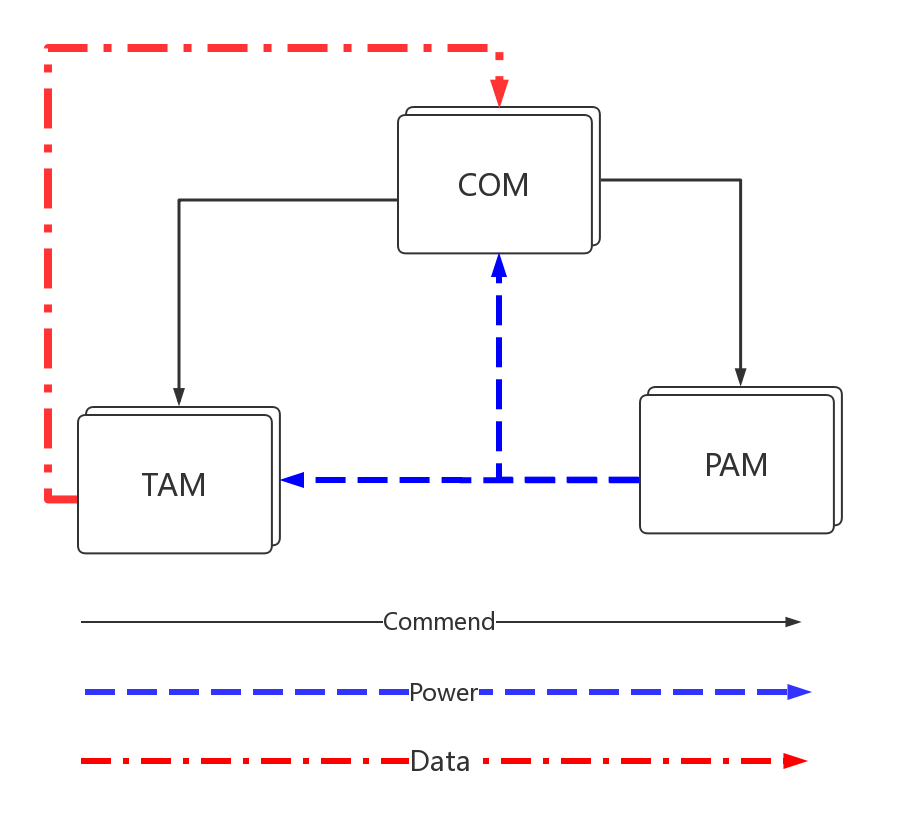
\includegraphics[width=\textwidth]{img/ES00003_Globaldia.png}
 \caption{System Diagram}	
\end{figure}
\clearpage
\section{Payload Catalog}

\subparagraph{Critical Payload}
All the critical payload will be in the assigning unit.
\begin{itemize}
\item 4 low temp sensors for electronics \textbf{In each unit}
\item 4 low temp sensors for batteries \textbf{In power manager unit}
\item 4 current sensors for pyros \textbf{In actuator power unit}
\item 4 current sensors for batteries \textbf{In power manager unit}
\item 4 deployment sensors \textbf{In actuator power unit}
\item 4 actuator sensors \textbf{In actuator power unit}
\item 3 axis IMU \textbf{In main control unit and failure recovery unit}
\item 1 barometer  \textbf{In main control unit and failure recovery unit}
\end{itemize}

\subparagraph{Low Speed Payload}
All the low speed payload will be in the low speed sensor unit.
\begin{itemize}
\item 4 high pressure sensors for propulsion system
\item 2 low pressure sensors for pitot tube
\item 4 high temp sensors for propulsion system
\item 4 low temp sensors for electronics
\item 4 low temp sensors for batteries
\item 2 low temp sensor for ambient
\end{itemize}

\subparagraph{High Speed Payload}
All the high speed payload will be in the high speed sensor unit.
\begin{itemize}
\item 9 axis IMU
\item GNSS
\item 4x cameras
\end{itemize}

\clearpage
\section{Computing and Operation Module (COM)}
\begin{figure}[htp]
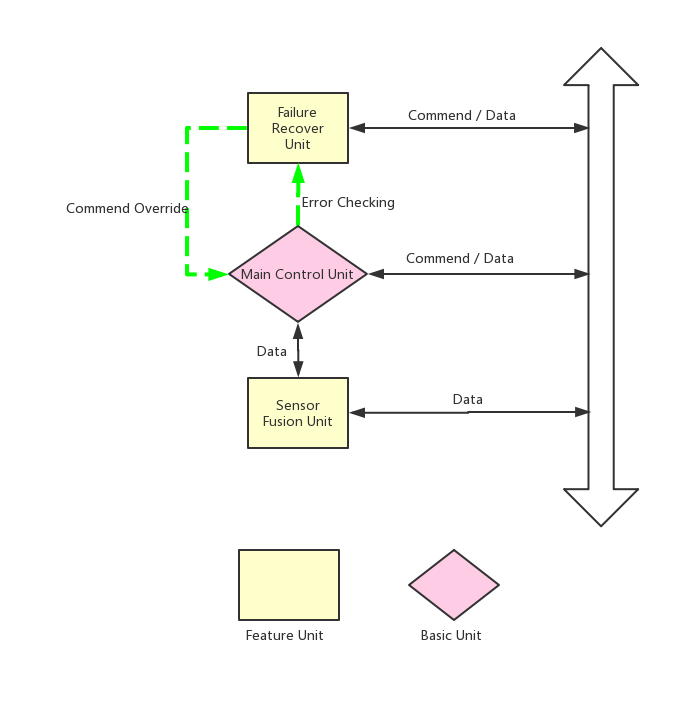
\includegraphics[width=\textwidth]{img/ES00003_COMdia.png}
 \caption{Computing and Operation Module Diagram}	
\end{figure}
\subsection{Main Control Unit (1)}
The main control unit will execute all the critical process during the whole launch. It will send commend via a commend lane to other module main unit to proform action. \textbf{This unit is require for all the OA-II VEH system.}
\subsection{Failure Recover Unit (2)}
The failure recover unit will execute similar code as the main control unit and detect any error that send out from the main control unit. When main control unit have error, it will inquire the main unit and check the answer. If a failure scenario is fullfill, it will take over the commend line and try to fix the problem by the program storage inside.
\subsection{Sensor Fusion Unit (3)}
The sensor fusion unit will communicate with the TAM and analyze the data. It will provide to the main control unit for more information.\\
\textit{\textbf{This unit will be include in the improved version.}}
\clearpage
\section{Telecommunication and Acquisition Module (TAM)}
\begin{figure}[htp]
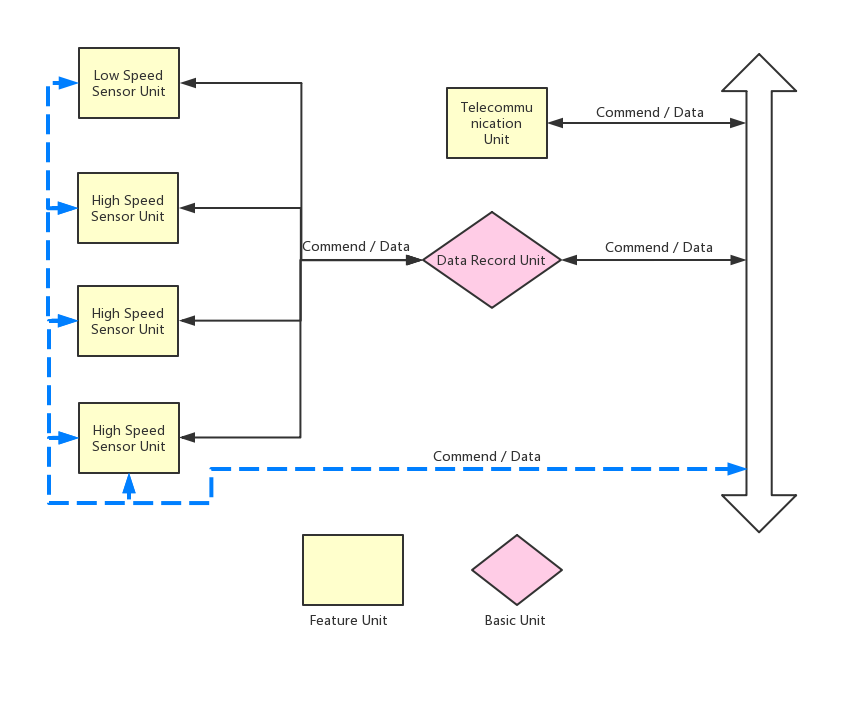
\includegraphics[width=\textwidth]{img/ES00003_TAMdia.png}
 \caption{Telecommunication and Acquisition Module Diagram}	
\end{figure}
\subsection{Data Record Unit (1)}
The data record unit is use to record log and data which send from the COM control. It will also include additional protection for protect storage unit from heavy impact.
%The data record unit is use to collecting data from the rest of the sensor unit in the module and provide to COM and telecommunication unit. It also will back up all the data to a storageto the media for recover after landing.
\subsection{Telecommunication Unit (2)}
The telecommunication unit is use to collect data from the record unit and send it down to the base station. It also will get commend that send from the base station and relay it to the COM.
\subsection{Low Speed Sensor Unit (3)}
The low speed sensor unit is use to contain sensors that have less then 100MB/s data rate. This unit will also have memory to buffering some of the data. The power supply for this unit will be a low voltage line from the PAM.
\subsection{High Speed Sensor Unit (4)}
The high speed sensor unit will use to contain sensors that have more than 100MB/s (ex: camera) 
%It will have a special power line from the PAM and itself will have memory for buffing data.
\clearpage
\section{Power and Actuator Module (PAM)}
\begin{figure}[h]
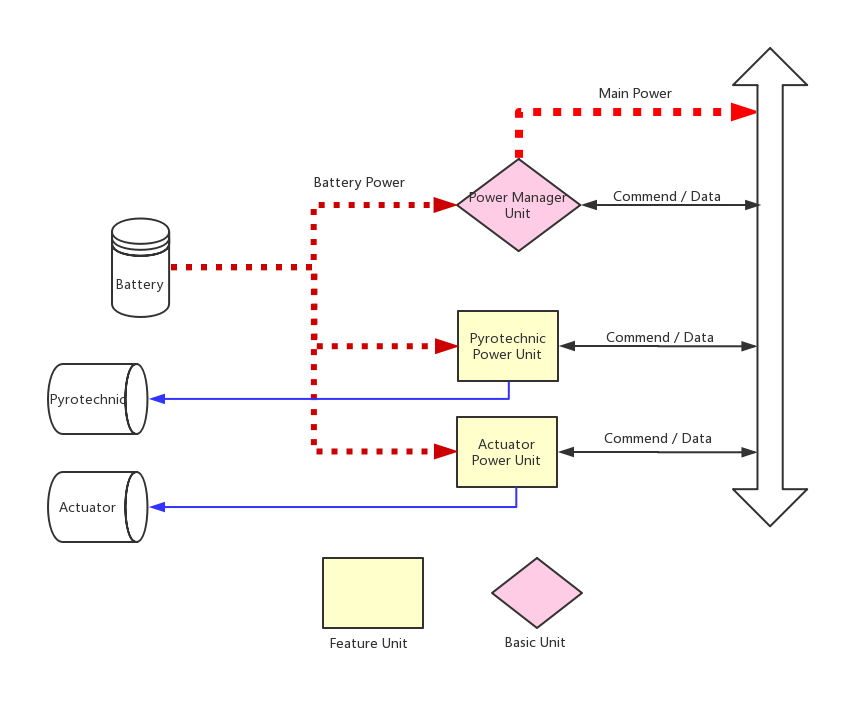
\includegraphics[width=\textwidth]{img/ES00003_PAMdia.png}
 \caption{Power and Actuator Module Diagram}	
\end{figure}
\subsection{Power Manager Unit (1)}
The power manager unit is use to control charge and discharge of the on unit main battery. It also have regulator to provide main rail power for the whole vehicle. \textbf{This unit is require for all the OA-II VEH system.}
\subsection{Pyrotechnic Power Unit (2)}
This unit contain spcial purpose voltage regulator and pyrotechnic driver. It will use to control the pyrotechnic device in the ship base on the commend come from the COM. 
\subsection{Actuator Power Unit (3)}
This unit contain spcial purpose voltage regulator and actuator driver. It will use to control the actuator in the ship base on the commend come from the COM.
\section{Product Code}
\begin{LARGE}
OA2-<COM/PAM/TAM>-XXX-[YY-Z]
\end{LARGE}\\\\
\subparagraph{XXX}
The first letter is indecate which kind of rocket it fit for. \textbf{H} for high power,\textbf{N} for general purpose, \textbf{S} for small scale. The number follow it is depend unit. The last number is what this unit belongs to. 
\subparagraph{YY}
Designer name.
\subparagraph{Z}
Revision number.\\\\
example: 
\begin{large}
OA2-COM-N01-[JC-1]
\end{large}\\\\
First generation Computing and Operation Module main unit design by Jinzhi Cai.
\newpage
\chapter{Revision History}% ; change PAM unit describtion
\begin{table}[H]
	\centering
	\begin{tabu}{r || c | c | c }
		Rev\# & Editor & Delta & Date\\ \hline
		A01 & Jinzhi Cai & Initialize  & 2019-7-2\\
		- & Jinzhi Cai & change name from "board" to "unit" & 2019-7-3\\
		- & Jinzhi Cai & change product code & 2019-7-3\\ \hline
		A02 & Jinzhi Cai & change PAM unit describtion & 2019-7-3\\
		- & Jinzhi Cai & add diagram & 2019-7-3\\ \hline
		A03 & Jinzhi Cai & change DRU & 2019-7-8\\ \hline
		A04 & Jinzhi Cai & add sensors & 2019-7-16\\ \hline
	\end{tabu}
	\caption{Summary of Revision History}
	\label{tab:edatools}
\end{table}
% End of document.
%**********************************************************************
\end{document}